\documentclass[../main.tex]{subfiles}
 
\begin{document}

\begin{figure}[h]
  \bc
  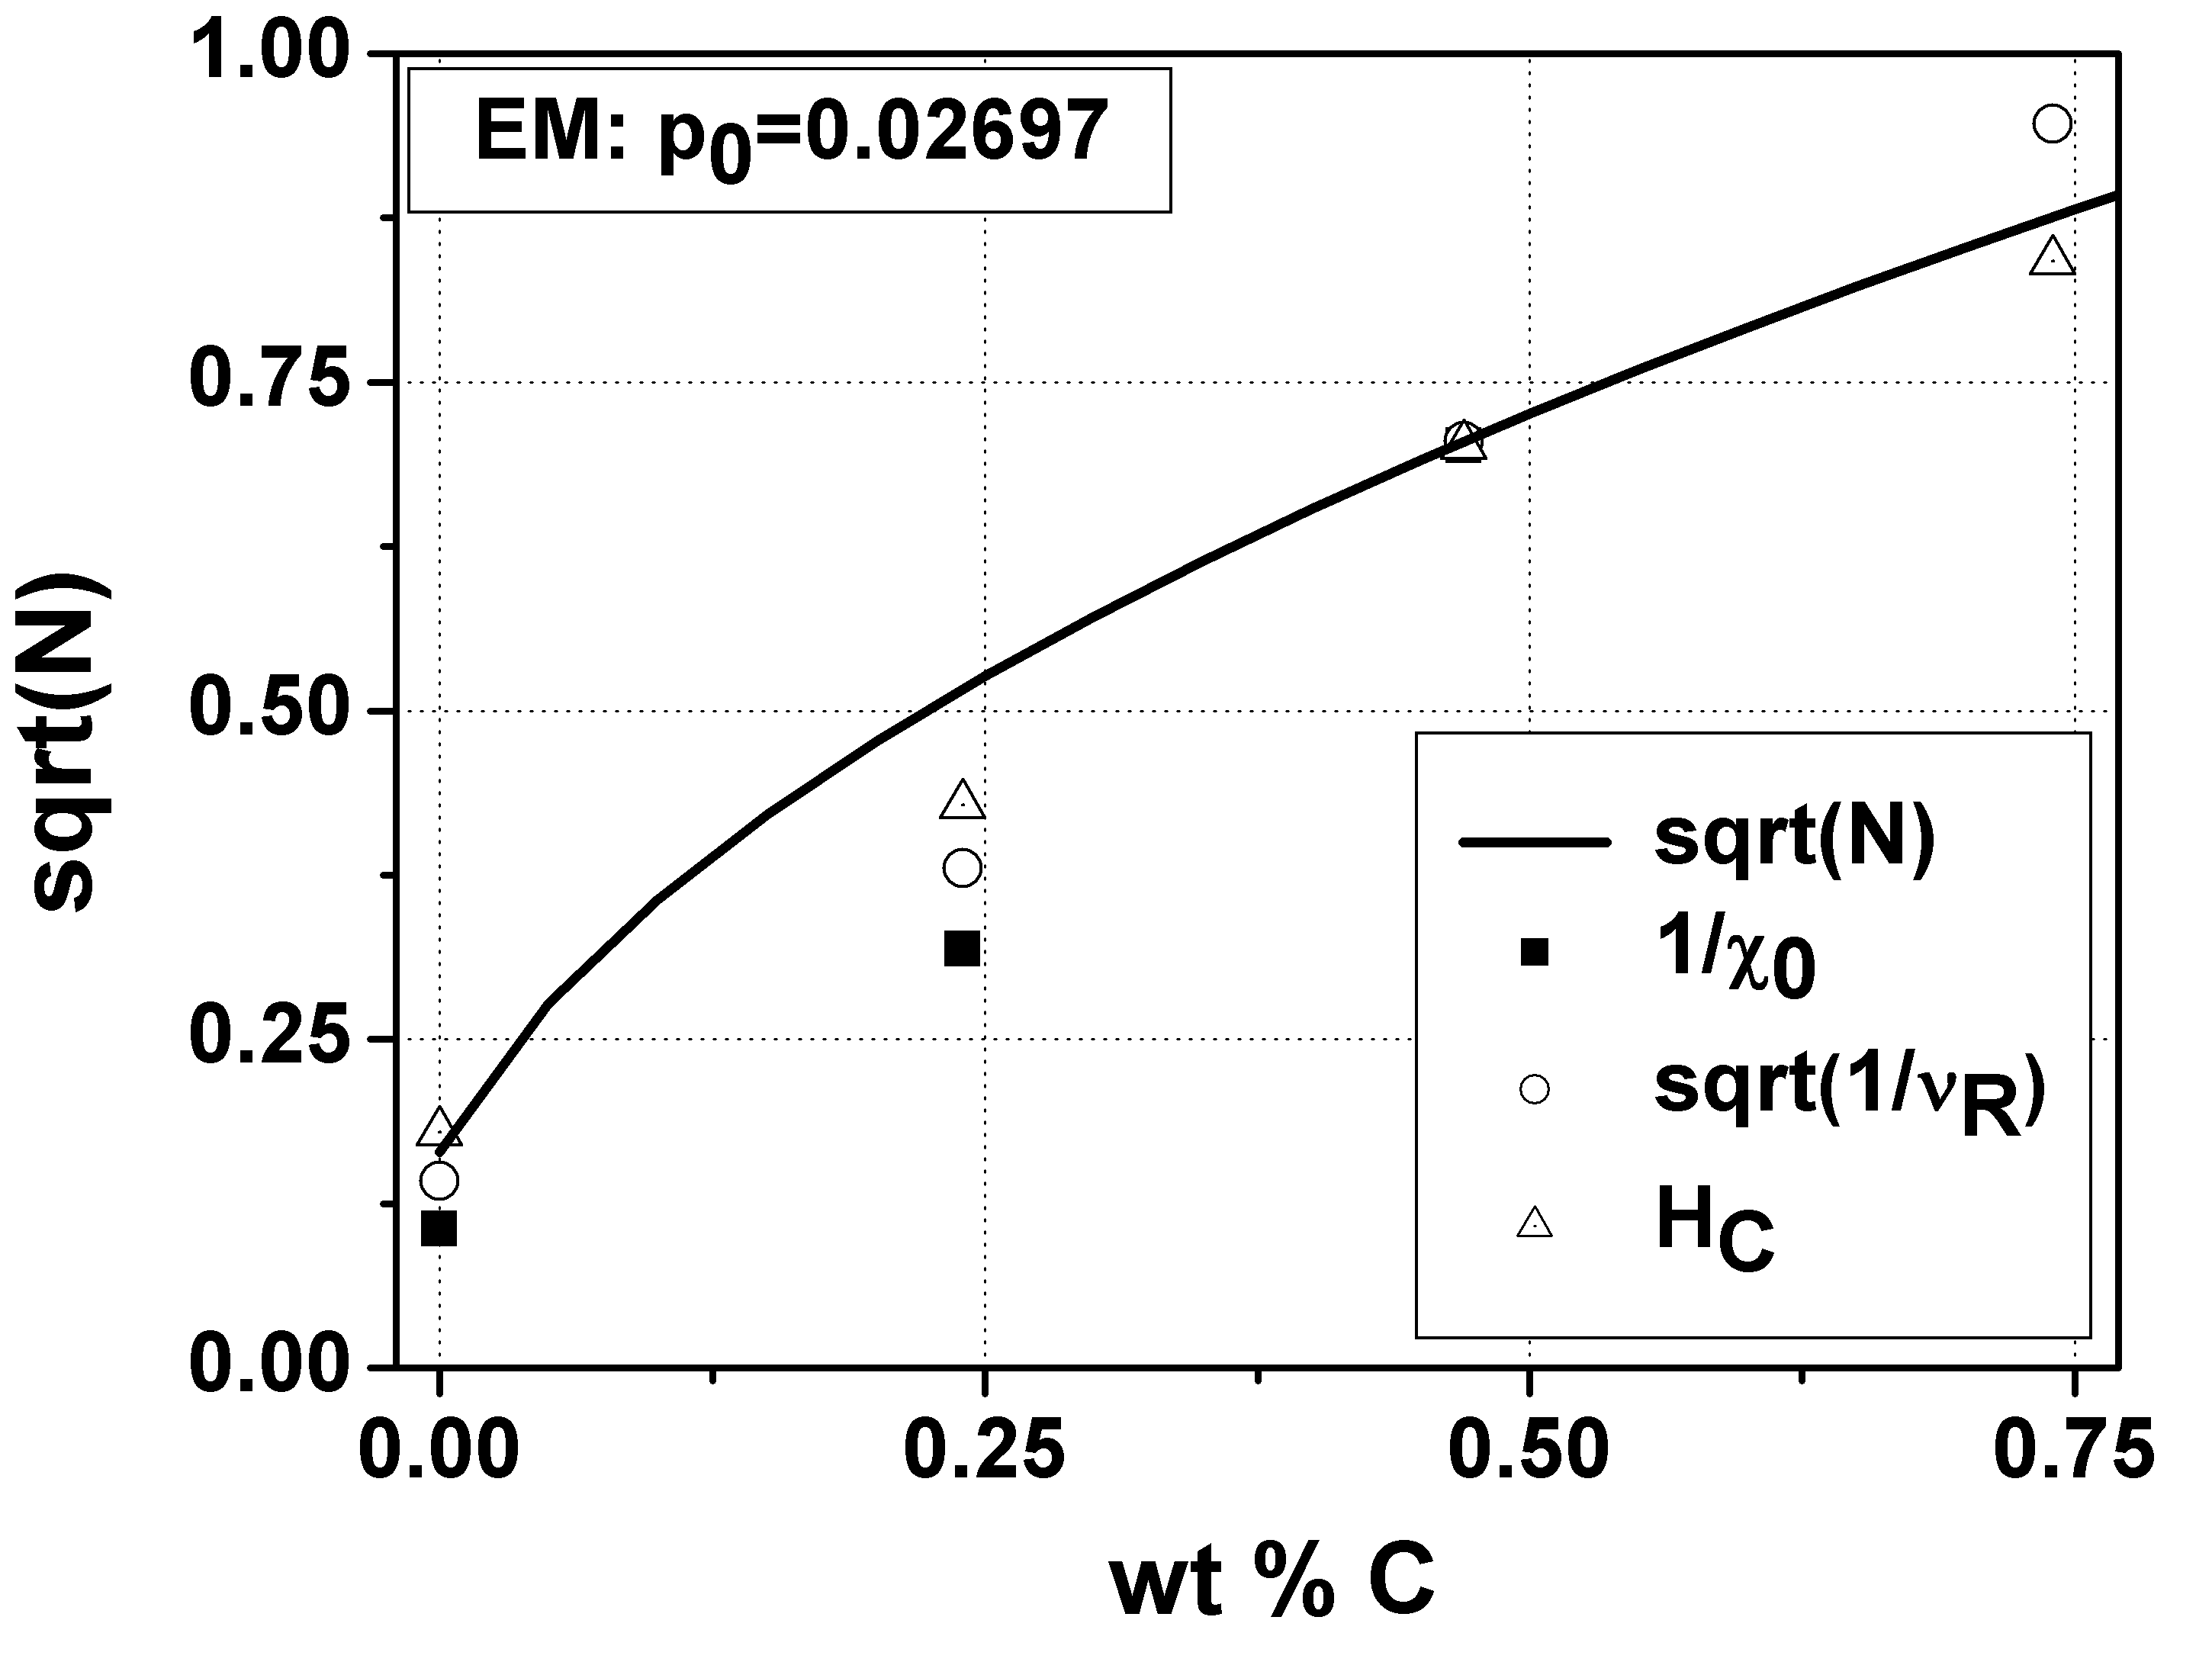
\includegraphics[width=0.7\textwidth]{HauserEtAl_Fig1.png}
  \ec
  \caption{\label{FigureEM}
  Normalized dependences of $1/\chi_0$, $\sqrt{1/\nu_R}$, $H_c$ calculated from EM
  and $\sqrt{N}=\sqrt{p_0+p_{\rm C}}$ as a function of wt \% C of Fe-C series.}
\end{figure}

\begin{figure}[h]
  \bc
  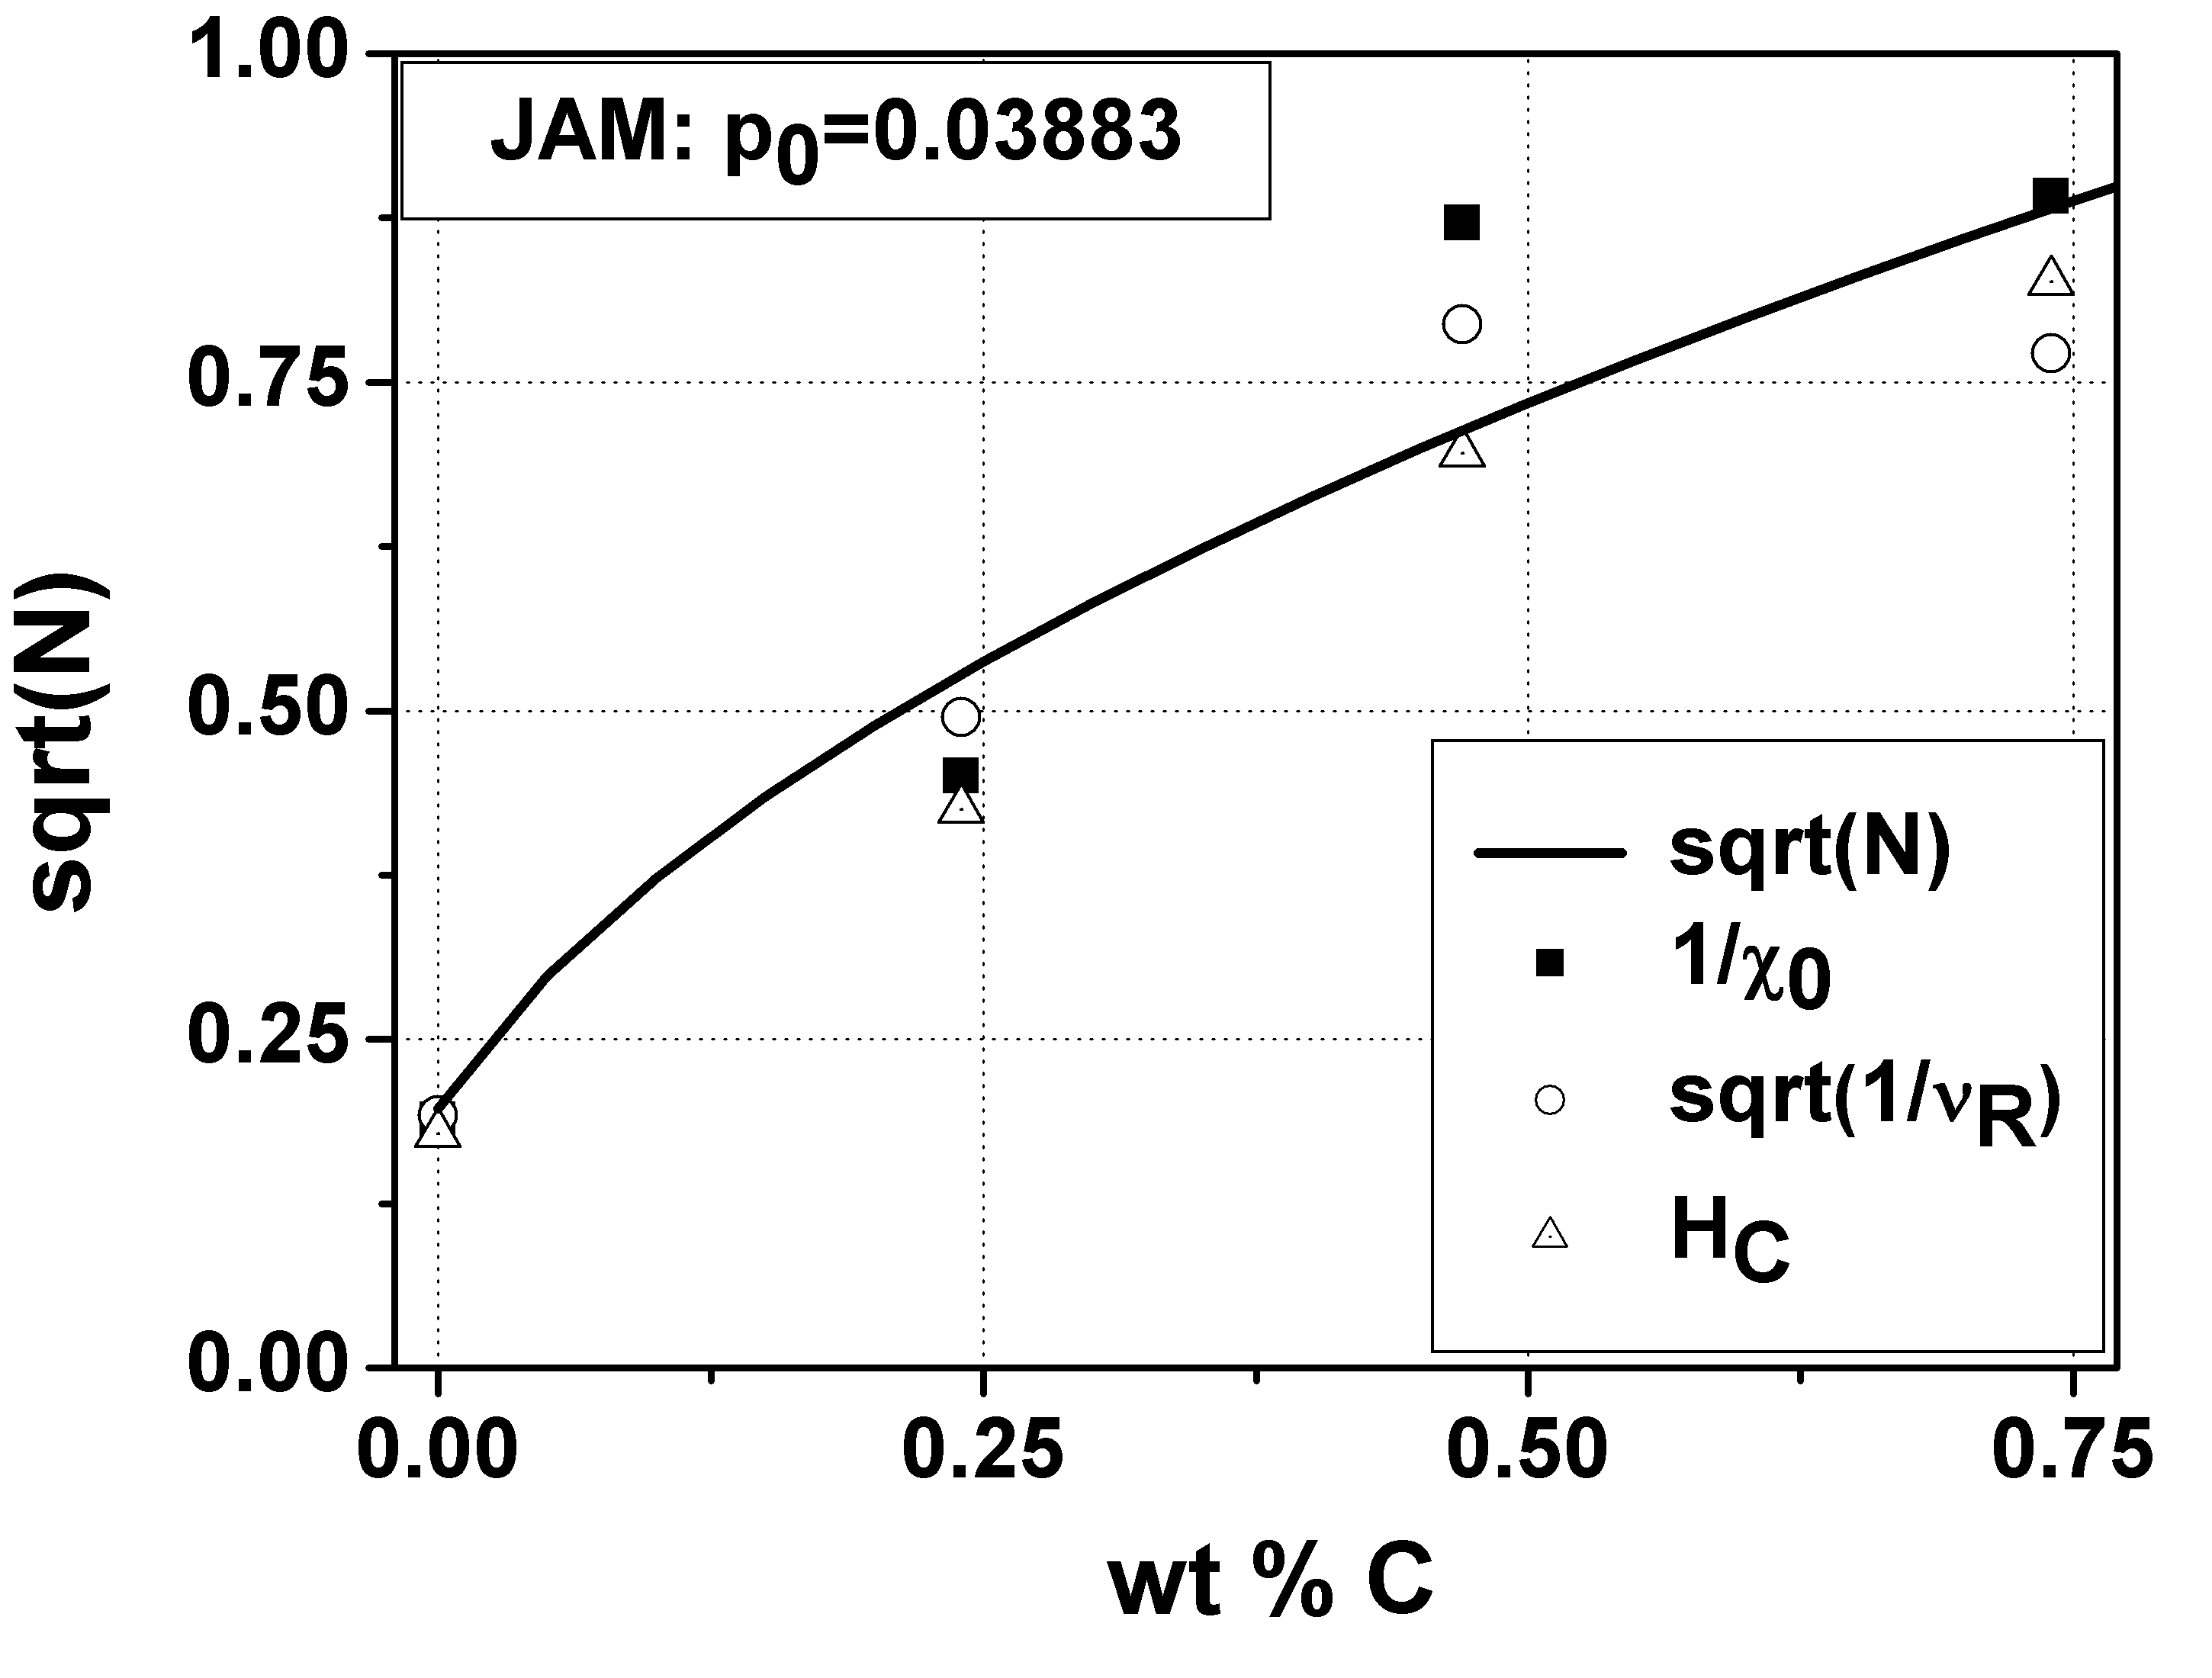
\includegraphics[width=0.7\textwidth]{HauserEtAl_Fig2.png}
  \ec
  \caption{\label{FigureJAM}
  Normalized dependences of $1/\chi_0$, $\sqrt{1/\nu_R}$, $H_c$ calculated from JAM
  and $\sqrt{N}=\sqrt{p_0+p_{\rm C}}$ as a function of wt \% C of Fe-C series.}
\end{figure}

\begin{figure}
  \bc
  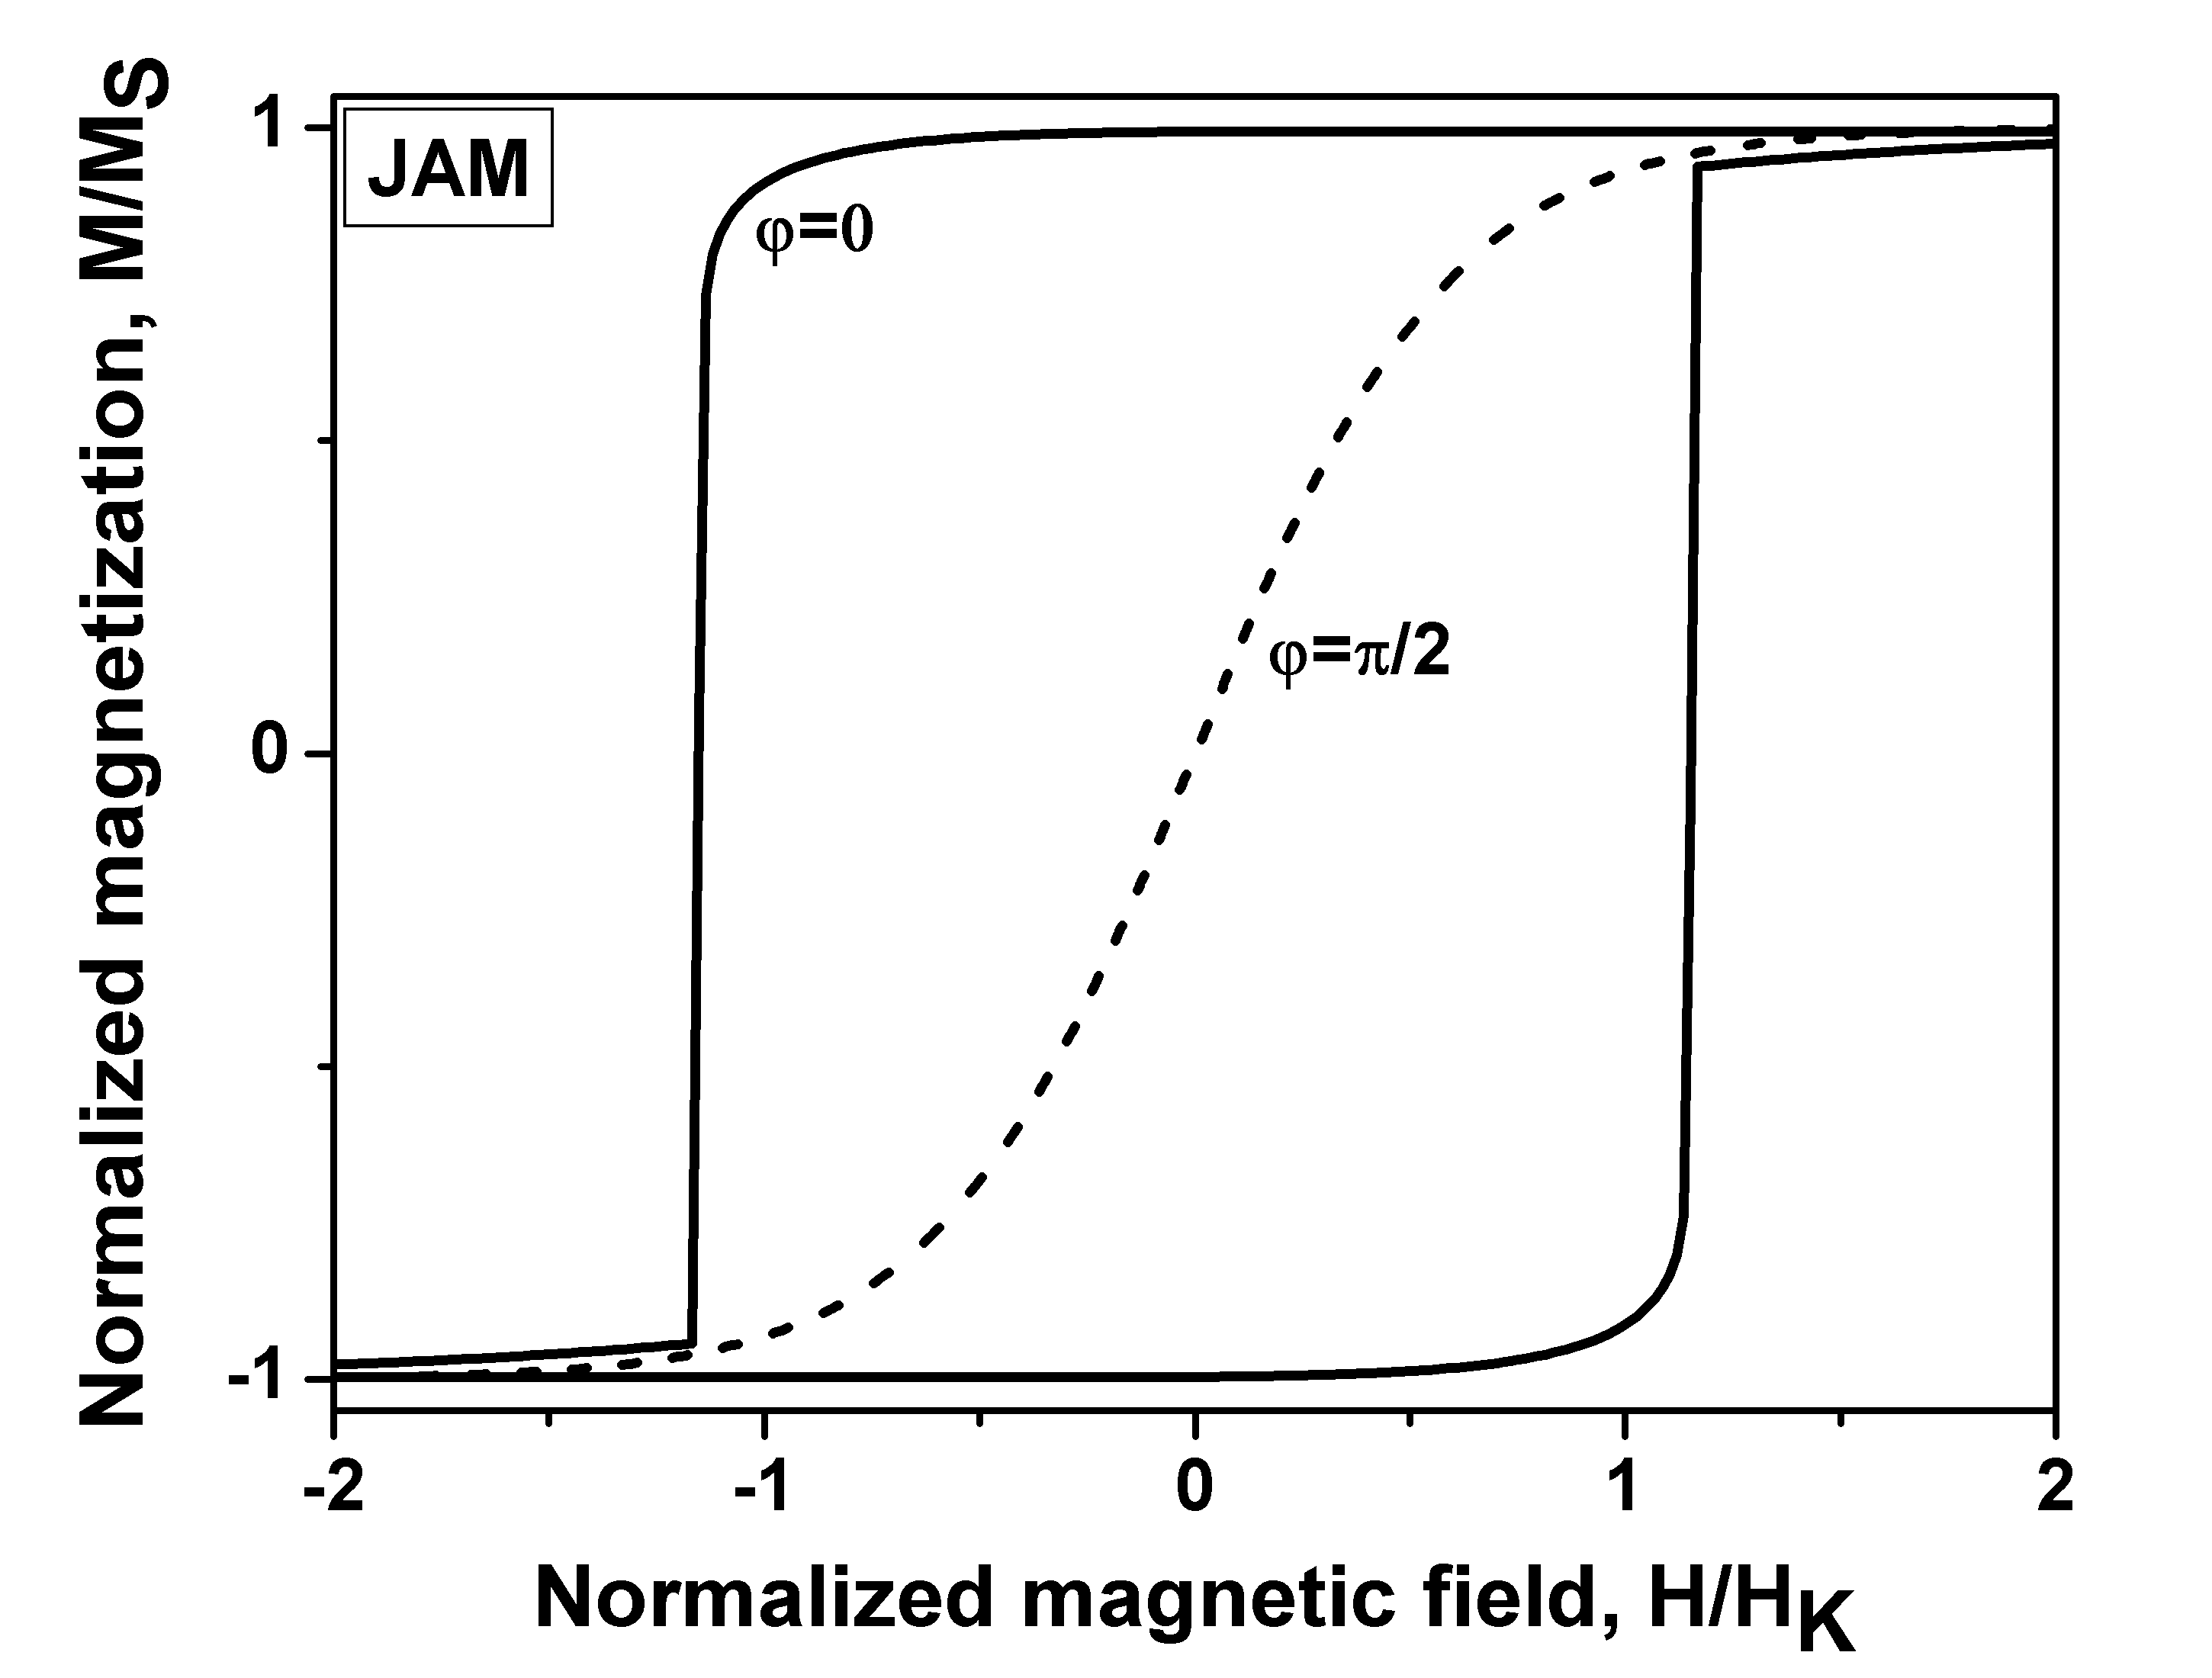
\includegraphics[width=0.7\textwidth]{HauserEtAl_Fig3.png}
  \ec
  \caption{\label{jmsw}
  SW-JAM hysteresis simulations of $\varphi=0$ 
  (with $M_s=800$~kA/m, $a=6$~kA/m, $k_J=10$~kA/m, $\alpha=0.02$, $c=0$ and $N_d=0$) and
  $\varphi=\pi/2$
  (with $M_s=800$~kA/m, $a=6$~kA/m, $k_J=0.01$~A/m, $\alpha=0.0$, $c=1$ and $N_d=0$)
  with $H_k=10$~kA/m. }
\end{figure}

\begin{figure}
  \bc
  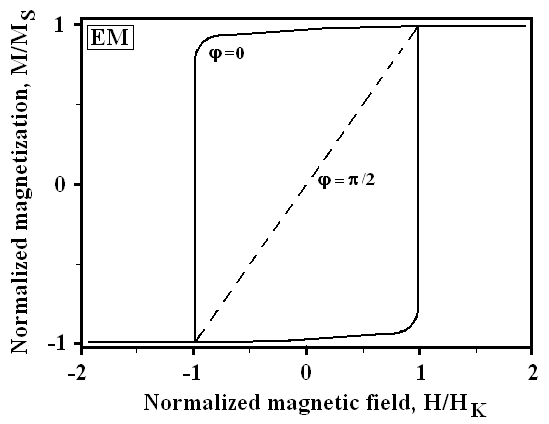
\includegraphics[width=0.7\textwidth]{HauserEtAl_Fig4.png}
  \ec
  \caption{\label{emsw}
  SW-EM hysteresis simulations of
  $\varphi=0$ (with $M_s=800$~kA/m, $g=120$, $h=10^{-33}$, $k_H=10$~kJ/m$^{3}$ and $q\gg1$) and
  $\varphi=\pi/2$ (with $M_s=800$~kA/m, $g=120$, $h=10^{-33}$, $k_H=10$~kJ/m$^{3}$ and $q=0$)
  with $H_k=10$~kA/m. }
\end{figure}

\cleardoublepage

\end{document}